\documentclass[../SimBALink.tex]{subfiles}
\graphicspath{ {../Model/Powertrain/Battery_pack/Documentation/Figures/Validation/}{./Model/Powertrain/Battery_pack/Documentation/Figures/Validation/}{./Model/Powertrain/Battery_pack/Validation/Figures/}{../Model/Powertrain/Battery_pack/Validation/Figures/} }

\begin{document}

\subsection{Battery pack model performance}
	The battery pack model was calibrated against discharge data from three sample cells. The model, with the calibrated parameters, was simulated using a current profile representative of a competition load. The model output was compared to test data.
	\subsubsection{Calibration}
		The battery pack model was calibrated using data from two discharge tests.
		
		\paragraph{Open-circuit voltage}
			First, a low-rate discharge test was used to approximate the battery open-circuit voltage $V_\text{oc}(\text{SOC)}$. In this test, the battery was charged to a terminal voltage of 4.2 V (constant-voltage, C/20 cutoff), then discharged at 0.1C until the terminal voltage reached 2.5 V.  
			
			Figure \ref{fig:0.1C_Discharge_Voltage_Profile} shows an example of 0.1C discharge test voltage data. The test was repeated three times on a sample cell at 20\degree C.
		
			\begin{figure}[h!]
				\centering
				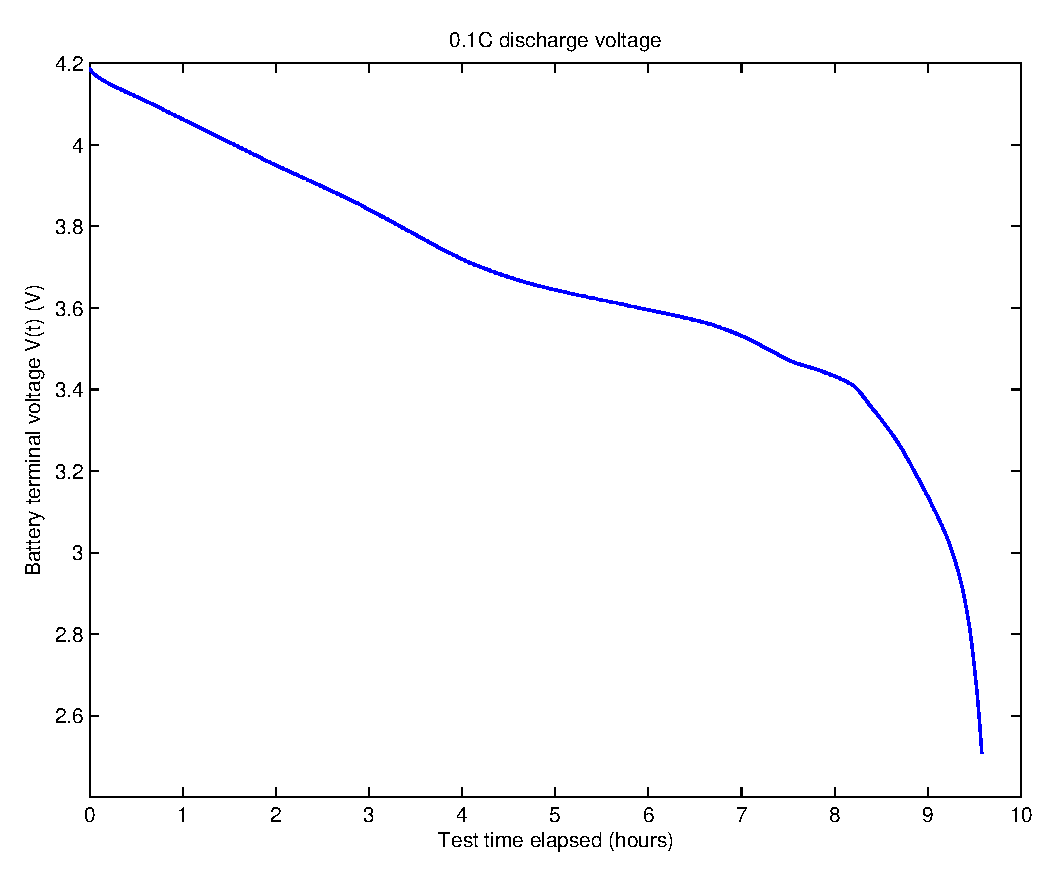
\includegraphics[width=5in]{1dC_Discharge_Voltage_Profile}
				\caption{Battery open-circuit voltage discharge test - voltage profile}
				\label{fig:0.1C_Discharge_Voltage_Profile}
			\end{figure}
		
			The actual current out of the cell recorded during testing was integrated to calculate the capacity discharged as a function of time. Equation \ref{eqn:SOC} gives the expression of battery state-of-charge, where $C$ is the battery capacity in amp-hours, and $I(T)$ is the measured discharge current from the cell, in amps.
		
			\begin{gather}
				C = \int_0^{t_\text{end}} \! I(T) \, \mathrm{d}T				\\
				\text{SOC}(t) = 1 - \frac{1}{C} \int_0^{t} \! I(T) \, \mathrm{d}T
				\label{eqn:SOC}
			\end{gather} 
		
			$\text{SOC}(t)$ and $V(t)$, the measured terminal voltage of the cell, were used to create a 1D lookup table of the cell's open-circuit terminal voltage.
			
			\FloatBarrier
			
		\paragraph{Equivalent-circuit parameters}
			After the open-circuit voltage had been calibrated and loaded into the model, data from a pulse discharge test was used to calibrate the equivalent-circuit parameters $R_0$, $R_1$, and $C_1$. The discharge test current profile, shown in Figure \ref{fig:Pulse_Discharge_Current_Profile}, consists of sets of high-magnitude current pulses at different states of charge.
			
			\begin{figure}[h!]
				\centering
				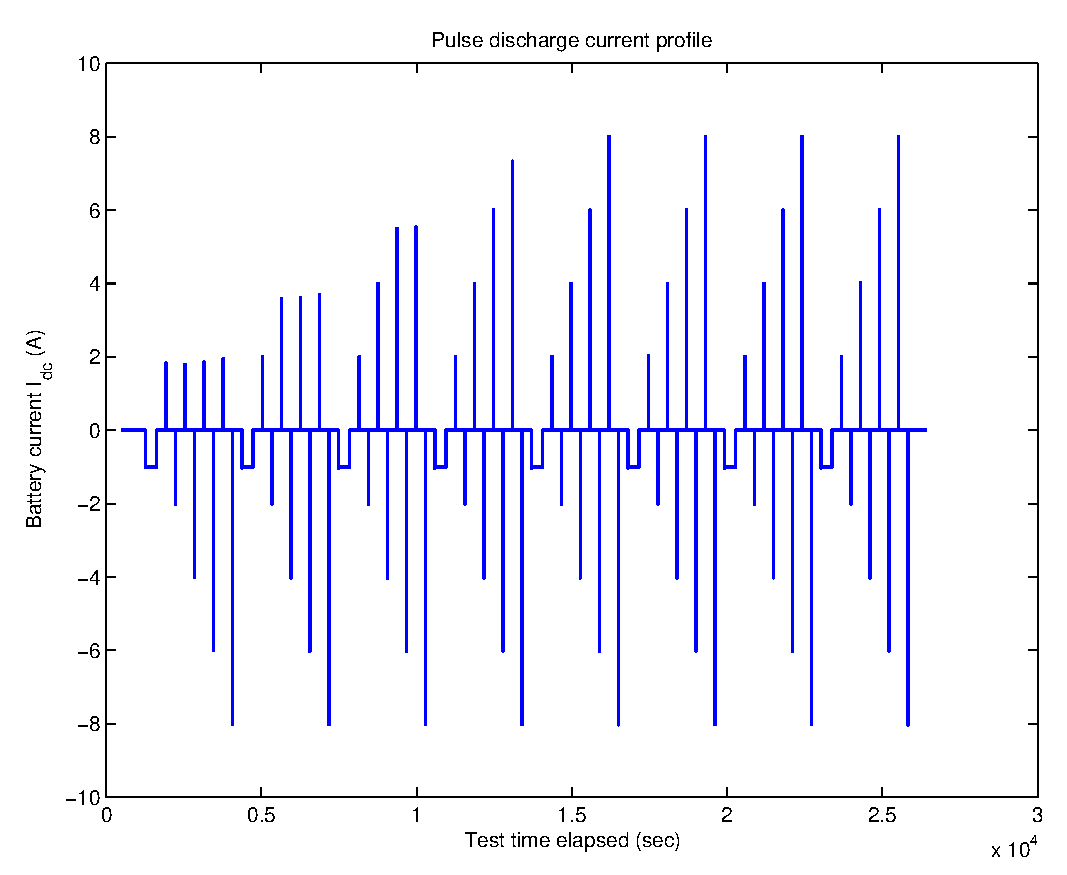
\includegraphics[width=5in]{Pulse_Discharge_Current_Profile}
				\caption{Pulse discharge test - battery current profile}
				\label{fig:Pulse_Discharge_Current_Profile}
			\end{figure}
			\FloatBarrier
			
			Using the discharge current profile in Figure \ref{fig:Pulse_Discharge_Current_Profile}, the model parameters in Table \ref{table:battery_calibrated_parameters} were calibrated using the MATLAB \texttt{fminsearch()} function.
			
			\begin{table}
				\centering
				\caption{Calibrated parameters in battery pack model}
				\label{table:battery_calibrated_parameters}
				\begin{tabular}{c | l | c | c}
					Symbol		&	Parameter			&	Initial guess value	&	Calibrated value	\\
					\hline
					$R_0$		&	Zero-order resistance	&	25 m$\Omega$	&	24.5 m$\Omega$	\\
					$R_1$		&	First-order resistance	&	25 m$\Omega$	&	24.1 m$\Omega$	\\
					$C_1$		&	First-order capacitance	&	1000 farad		&	982.9 farad		\\
					$R_0$		&	Capacity				&	2.5 Ah			&	2.35 Ah
				\end{tabular}
			\end{table}
			\FloatBarrier
			
			The capacity parameter was included as a calibrated parameter because initial tests with the model displayed what appeared to be a scaling error in the model's open-circuit voltage term.
			
	\subsubsection{Model validation and quality of fit}
		\begin{figure}[h!]
				\centering
				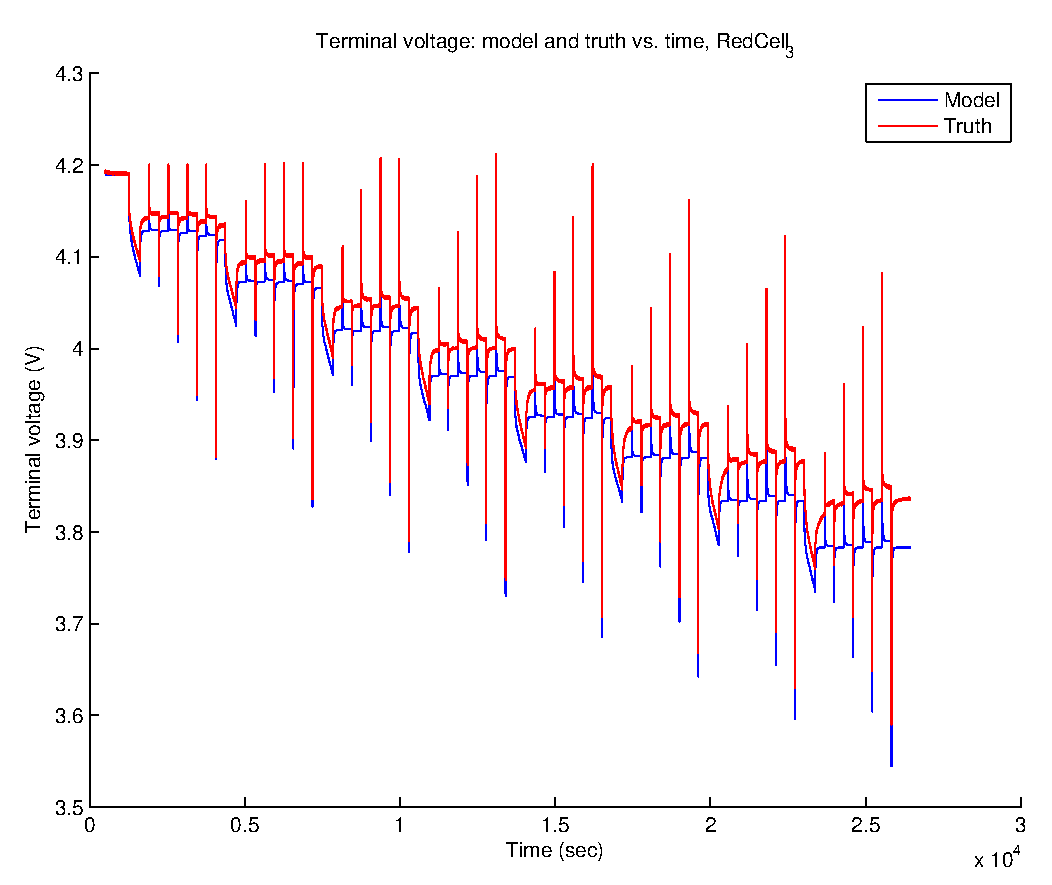
\includegraphics[width=5in]{ModelAgreement_RedCell_3_Pulse}
				\caption{Model agreement - pulse discharge profile}
				\label{fig:Pulse_Discharge_Current_Validation}
			\end{figure}
		
		Figure \ref{fig:Pulse_Discharge_Current_Validation} shows the model behavior compared to a pulse discharge test for a different cell. Although the dynamic response of the circuit (RC network) is close to accurate, the open-circuit behavior with SOC displays increasing error as the test continues (and cell state-of-charge decreases).
		
		Measurement error is a likely source of this issue. In Jan. 2014, the calibrations will be repeated with more precise equipment and a larger sample size.
		
		
\end{document}